\pdfoutput=1
\documentclass[11pt]{article}
\usepackage[margin=1in]{geometry}
\usepackage{amsmath,amssymb,amsthm}
\usepackage{enumitem}
\usepackage{booktabs}
\usepackage{longtable}
\usepackage{array}
\usepackage{tikz}
\usetikzlibrary{arrows.meta,positioning,shapes.geometric}
\usepackage{hyperref}
\hypersetup{hidelinks,
  pdftitle={A conditional assembly from Theorem 3.11 to Corollary 3.12: decomposition of the scalar layer, a semantic principle, and isolation of the value-group profile switch},
  pdfauthor={Toshihisa Urahigashi}}

\newcommand{\cO}{\mathcal O}
\newcommand{\cU}{\mathcal U}
\newcommand{\cK}{\mathcal K}
\newcommand{\uu}[1]{\underline{\underline{#1}}}
\newcommand{\stmt}[2]{\medskip\noindent\textbf{#1\ #2.}\ }
\newcommand{\pf}{\medskip\noindent\textit{Proof.}\ }
\newcommand{\pfs}{\medskip\noindent\textit{Sketch of proof.}\ }
\newcommand{\qedh}{\hfill\(\square\)\par\medskip}

\title{A conditional assembly from Theorem~3.11 to Corollary~3.12:\\
decomposition of the scalar layer, a semantic principle,\\
and isolation of the value-group profile switch}
\author{Toshihisa Urahigashi\\
\small\texttt{123026.urahigashi.toshihisa@gmail.com}}
\date{Version 1.0.1 --- 13 November 2026\\[3pt]
\small Independent researcher. This work was carried out personally and is
unrelated to any institutional affiliation.\\[3pt]
\small ORCID \href{https://orcid.org/0009-0004-0460-6242}{\texttt{0009-0004-0460-6242}}\\[-2pt]
\small \href{https://doi.org/10.5281/zenodo.24179190}{doi:10.5281/zenodo.24179190} (all versions: \href{https://doi.org/10.5281/zenodo.24166924}{10.5281/zenodo.24166924})}

\begin{document}
\maketitle

\begin{abstract}
We report a \emph{conditional assembly} of the passage from
Theorem~3.11 to Corollary~3.12 in inter-universal Teichm\"uller
theory (IUT), expanding the seams that the source treats by
abbreviation conventions and citations to numbered results.  This
paper does not claim an unconditional proof of Corollary~3.12 or of
the ABC conjecture.  The claim has the following form: accept the
numbered statements of IUT~I--IV as black boxes, take Mochizuki's
non-IUT papers ([FrdI], [FrdII], [EtTh], [AbsTopIII], etc.) and
classical results as known inputs, accept a single semantic
principle~S (prime-strip isomorphisms are isomorphisms of
collections of data intertwining all constituents, and compatibility
is read as commutative squares), and moreover accept, as an explicit
input, the central value-group switch \textbf{H*val} (hull
compatibility of the switch from $\Psi_{\mathrm{LGP}}$ to $\Psi_q$);
then each step of the passage is filled by named grounds.  The
scale-preservation problem is decomposed into local cancellation,
chart transport (distortion $=1$), an explicit formula for the
mono-analytic correction, distortion of evaluation isomorphisms, and
mutual compatibility of cyclotomic rigidities.  Of these, the
\emph{scalar layer} --- chart calibration, generator scalars and
transport distortion --- is supplied at the statement level using
material outside the cited range; this is a part that was not
derivable in the cited theory of [U26].  An external adjudication
has however settled that the loop argument of Lemma~8.1 proves only
identity of the chart calibration for the two routes, not equality
of pilot profiles.  The value-group switch therefore remains
unresolved, as the core of strong (SHE)/(9-1).  Sufficiency of the
assembly is also machine-checked in Lean~4 (the capstone
\texttt{cor312\_of\_assembly}, standard three axioms only in the
recorded selected build).  What remains is the IUT black box itself,
the value-group switch H*val, inhabitation of Principle~S in the
actual construction (frame fidelity), and independent re-verification
of this paper.  The correspondence with preceding reductions (the
Scholze--Stix critique, Project LANA's (9-1) and \texttt{xi\_iff}) is
also made explicit.

The difference from the author's preceding work [U26], \emph{Where
Theorem 3.11 sits}, is stated at the outset.  What [U26] proved is
negative: from the statements actually cited in the proof of
Corollary~3.12 alone, Corollary~3.12 does not follow (a countermodel
exists).  The present paper works in the opposite direction: using
the content of the actual construction outside the cited range, it
assembles the passage at the statement level (the level at which
numbered statements are used as black boxes and the seams between
them are filled by expanding definitions).  In the author's view,
many of the seams written out here may correspond to parts that were
present in the IUT author's mind but were not written down, inside
the proof of Corollary~3.12, as citable statements; the work of this
paper may be read as an attempt to supply that unwritten layer.
This is the author's interpretation, not a claim about the IUT
author's intentions.

\smallskip
\noindent\emph{Keywords:} inter-universal Teichm\"uller theory,
Corollary~3.12, scale preservation, multiradial representation,
completeness, formalization (Lean), cyclotomic rigidity.
\end{abstract}

\medskip
\noindent\textbf{Note added in version 1.0.1.}
This version only adds the caution note on Figure~1 below: the Venn
diagram in Figure~1 is currently misrendered.  No text, result or
conclusion is changed.

\section*{Claim and what remains, at the outset}

The claim of this paper is that what have been treated as ``walls''
--- Corollary~3.12, the height inequality, LANA's (9-1) --- have
been reduced to the following list of remaining items.  If all of
them are established, Corollary~3.12 follows, and through the
machinery of IUT~IV an ABC-type height inequality follows.

In relation to the preceding work: of what was underivable in [U26],
the \emph{scalar layer} (chart calibration, generator scalars,
transport distortion) is supplied in this paper, and what remains at
the centre is the \emph{profile layer}.  Supplying the scalar layer
does not by itself mean that the aggregate defect $\Delta$ vanishes.
The step that carries a raw $\Theta$-pilot profile to a $q$-pilot
representation remains as item R2V below.

\begin{itemize}[leftmargin=*]
\item \textbf{(R1) The IUT black box.}  Correctness of the numbered
  statements of IUT~I--IV, including Theorem~3.11.  Not verified
  here.
\item \textbf{(R2V) The value-group switch H*val.}
  The switch $\Psi_{\mathrm{LGP}}\to\Psi_q$ is compatible with the
  holomorphic hull, and an actual $q$-pilot representation is
  obtained from the $\{j^2u_{\underline v}\}_j$-type $\Theta$-pilot
  profile.  Lemma~8.1 proves only that the two routes give the same
  $\Phi^{\mathrm{rlf}}$ chart calibration; Lemma~8.2 treats only the
  unit side.  This is the core of strong (SHE)/(9-1) (\S8).
\item \textbf{(R2) Inhabitation of Principle~S in the actual
  construction.}  Each isomorphism that the source calls a
  prime-strip isomorphism (evaluation, Kummer, links), also in
  situations where the same object is identified in other ways,
  satisfies the two commutative squares and non-degeneracy as a
  morphism in the sense of Definition~5.2 (in Lean: inhabitation by
  the actual objects of \texttt{TwoSquareFVdashIso} = frame
  fidelity).  The phenomena already reproduced in models and the
  precise transfer problem to the actual construction are detailed
  in \S3.1.
\item \textbf{(R3) Independent re-verification of this paper.}
  Not a mathematical hypothesis but work not yet done, including
  completeness of the enumeration of seams.
\item \textbf{(R4) Only for explicit ABC constants.}
  Numerical values of $B_{\cK}^{*}$ for concrete $\cK_V$ (computable
  from the definition; a finite example is in \S11) and treatment of
  the coefficient case $(\ell,d_{\mathrm{mod}})=(5,1)$.  Not needed
  for Corollary~3.12 itself.
\end{itemize}

Conversely, the content of the assembly in this paper is that no
input other than these is needed.  Figure~\ref{fig:venn} updates the
Venn diagram of [U26] to the present state.

\medskip
\noindent\textbf{Note on Figure~1 (misrendering).}
The Venn diagram in Figure~1 is currently misrendered: some labels
overlap or overflow.  The figure will be corrected in a later
version; for the present version, please rely on the caption rather
than the diagram itself.

\begin{figure}[ht]
\centering
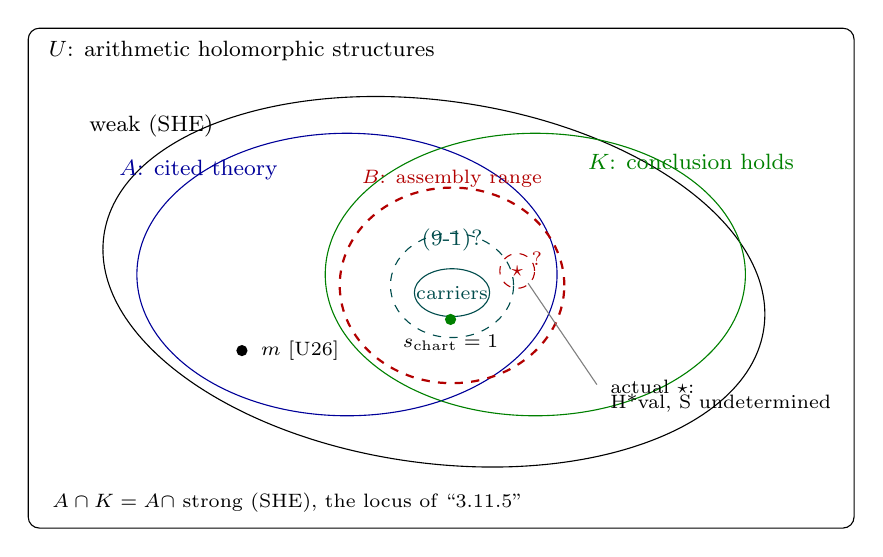
\begin{tikzpicture}[scale=0.92, every node/.style={font=\footnotesize}]
  \draw[rounded corners] (0,0) rectangle (11.4,6.9);
  \node[anchor=north west] at (0.15,6.85) {$U$: arithmetic holomorphic structures};
  \draw[rotate around={-8:(5.6,3.4)}] (5.6,3.4) ellipse (4.6 and 2.5);
  \node at (1.7,5.55) {weak (SHE)};
  \draw[blue!60!black] (4.4,3.5) ellipse (2.9 and 1.95);
  \node[blue!60!black] at (2.35,4.95) {$A$: cited theory};
  \draw[green!50!black] (7.0,3.5) ellipse (2.9 and 1.95);
  \node[green!50!black] at (9.15,5.05) {$K$: conclusion holds};
  \fill (2.95,2.45) circle (2.2pt);
  \node[anchor=west,font=\scriptsize] at (3.08,2.45) {$m$ [U26]};
  \draw[red!70!black,dashed,thick] (5.85,3.35) ellipse (1.55 and 1.35);
  \node[red!70!black,font=\scriptsize] at (5.85,4.82) {$B$: assembly range};
  \draw[teal!60!black,dashed] (5.85,3.35) ellipse (0.85 and 0.72);
  \node[teal!60!black] at (5.85,3.98) {(9-1)?};
  \draw[teal!60!black] (5.85,3.25) ellipse (0.52 and 0.33);
  \node[teal!60!black,font=\scriptsize] at (5.85,3.25) {carriers};
  \fill[green!50!black] (5.83,2.88) circle (2.2pt);
  \node[font=\scriptsize,anchor=north] at (5.83,2.80) {$s_{\mathrm{chart}}=1$};
  \draw[red!70!black,dashed] (6.75,3.55) circle (0.24);
  \node[red!70!black] at (6.75,3.55) {$\star$};
  \node[red!70!black,font=\scriptsize] at (7.02,3.72) {?};
  \draw[gray] (6.90,3.38) -- (7.85,1.98);
  \node[anchor=west,font=\scriptsize] at (7.90,1.95)
    {actual $\star$:};
  \node[anchor=west,font=\scriptsize] at (7.90,1.72)
    {H*val, S undetermined};
  \node[anchor=west,font=\scriptsize] at (0.2,0.35)
    {$A\cap K=A\cap$ strong (SHE), the locus of ``3.11.5''};
\end{tikzpicture}
\caption{Updated Venn diagram: the diagram of [U26] with the
assembly range $B$ of this paper (dashed) superimposed (not to
scale).  Inside $A$ there still exists a countermodel $m$ where the
conclusion is false.  Using content outside the cited range
(expansions of definitions, explicit formulae, known literature),
the assembly builds the steps around (9-1) and the chart side of
$s=1$.  $B$ is not a range where (9-1) has been solved; it is the
range in which (9-1) has been isolated as the value-group switch
H*val (R2V).  Whether the star representing the actual construction
satisfies H*val and inhabitation of Principle~S (R2) is what
remains of the wall.  The IUT statements as a whole (R1) are a
premise outside the cited range defining $A$ in this figure.}
\label{fig:venn}
\end{figure}

\section{Introduction and position}

\textbf{Contrast with the preceding work.}  [U26] formalized the
range of statements cited in the proof of Corollary~3.12 and showed,
by a countermodel, that Corollary~3.12 does not follow from that
range alone.  The shortages localized there were, in the terminology
of the time, an input fixing the scale $s$, and uniformity in (IPL).
In this paper the former is further split into the \emph{scalar
layer} (chart calibration, generator scalars, transport distortion)
and the \emph{profile layer}, which concerns the arrangement of
value-group components.  As a sequel, this paper identifies step by
step where in the actual construction of the source the scalar layer
is supplied from, isolates the value-group switch at the centre of
the profile layer as a named remainder H*val, and assembles its
surroundings at the statement level.  The two are therefore not in
conflict: the countermodel of [U26] remains valid, and the assembly
here explicitly uses content outside the cited range (explicit
formulae, uniqueness characterizations, expansions of definitions).

\textbf{The author's interpretation.}  The seams expanded here ---
the explicit formula for the mono-analytic correction, computation
of distortion of evaluation isomorphisms, mutual compatibility of
cyclotomic rigidities, etc. --- are treated in the source by
abbreviation conventions, one-line proofs, and remarks.  In the
present author's view, these may correspond to parts that were
present in the IUT author's mind but were not written down, inside
the proof of Corollary~3.12, as citable statements; the work here
resembles an attempt to supply that layer.  Whether this
interpretation is apt is not part of the claims of this paper, and
whether the present assembly is correct as such a supplement awaits
independent re-verification.

The author's purpose is understanding of IUT, and this paper is work
of verification that reads through the IUT papers.  The mathematical
content is attributed to IUT~I--IV of Shinichi Mochizuki, the
founder of IUT; the contribution here is limited to making the seams
explicit and decomposing them into a verifiable form.  This paper
has not received confirmation or approval from Professor Mochizuki.

Corollary~3.12 of IUT~III, which derives the log-volume inequality
$-|\log(\uu\Theta)|\ge-|\log(\uu q)|$ from the multiradial
representation of Theorem~3.11, has been at the centre of the
controversy since 2018.  In [U26] we showed that axiomatizing only
the statements cited by Corollary~3.12 admits a countermodel, and
that an input fixing the scale $s$ and uniformity in (IPL) do not
exist inside the cited range.  In the sequel [U26b] the problem was
formulated as completeness for forgetful maps, and the sufficient
condition for ABC was reduced to the aggregate defect $\Delta$
(v1.1.3 clarifies that $\Delta$ is not a chart multiplier itself but
an aggregate quantity that may depend on the profile).  The main
countermodel of [U26] is not a model obtained by arbitrarily
stretching a chart.  It is a profile model with
$\theta_j=B(j,29j^2)$, $q_j=B(j,29)$, and
$s=3/14=12/(\ell(\ell+1))$ is an aggregate scalar forced as the mean
of that $j^2$ profile.  This paper is a sequel: using the content
of the actual construction outside the cited range, it identifies
where the scalar layer is supplied from, step by step, and isolates
the profile layer that still remains.

Priority for the reduction belongs to the Scholze--Stix critique and
to Project LANA.  In particular, LANA's (9-1) is the central
sentence corresponding to the value-group switch H*val isolated in
\S8 here, and this paper does not claim to have solved it.  The
dictionary is given in \S19 of the working draft [W].  The
contribution here is not a new mathematical idea but: (i) an
enumeration of seams with named grounds for each step; (ii) a rating
that includes the history of corrections of overstatements by
external cross-checking; (iii) an explicit finite list of remaining
dependencies, including H*val and in-situ inhabitation of
Principle~S; and (iv) machine verification of sufficiency in Lean.
The detailed proof material is in the working draft [W]
(ronbun9757); this note gives a summary and its position.  The
passage corresponding to Lemma~13.5 of [W]~v0.14 still needs
revision in line with the downgrade in \S8 here.

\medskip
\noindent\textbf{What this paper does not claim.}  An unconditional
proof of Corollary~3.12 or of the ABC conjecture; verification of
the correctness of IUT itself, including Theorem~3.11; or a rebuttal
of the Scholze--Stix critique.  This paper is a conditional assembly
--- ``if the listed inputs are accepted, the passage assembles'' ---
together with a complete explicit list of those inputs.

\section{Reduction to defect form and the Lean capstone}

Fix notation.  Let $v_{\mathrm{out}}=\mu^{\log}(T_\lambda)$ be the
global readout of the $\Theta$-link image $T_\lambda$ after transport
to a common $q$-side chart, and let
$v_Q=-|\log(\uu q)|$ be the volume of the input $q$-pilot.  The
scale $s\in\mathbb R_{>0}$ is defined by $v_Q=s\cdot
v_{\mathrm{out}}$, and the defect by
$\Delta=(s-1)v_{\mathrm{out}}$.  The old notation
$\operatorname{vol}\theta$ for the raw volume before transport is
not used here, since the readout side becomes ambiguous.  The
sufficient condition for the output hull $H$ reduces to two
sentences: the input sentence is exact scale preservation $s=1$
(i.e.\ $\Delta=0$); the output sentence is that the single global
object $T_\lambda$ belongs to the family of possible images and
$v_{\mathrm{out}}\le\operatorname{vol}H$.  As for signs: if
$\operatorname{vol}H\ge0$ then $v_Q<0\le\operatorname{vol}H$ and
the conclusion is trivial, so below $s>0$ is discussed on the
nontrivial region $\operatorname{vol}H<0$, in particular
$v_{\mathrm{out}}<0$.  This reduction and defect algebra are
verified in Lean~4, with the standard three axioms only.
\[
v_Q=s\cdot v_{\mathrm{out}},\qquad
\Delta=(s-1)v_{\mathrm{out}},\qquad
\Delta=0\iff s=1\ (v_{\mathrm{out}}\ne0),\qquad
\text{conclusion: }v_Q\le\operatorname{vol}H.
\]

The capstone \texttt{cor312\_of\_assembly} constructed in this work
(Lean; PASS on a selected closure) does not receive the input
sentence $s=1$ as a hypothesis; instead it derives it from
place-by-place equality of corrected volumes and a decomposition
into a common weighted sum.  The remaining hypotheses are made
explicit as three items --- volume decomposition (transport and
frame fidelity), corrected place-by-place equality, and the
membership sentence --- and are not axioms.  The Lean membership
hypothesis \texttt{hmem} is $T\in\mathrm{Fam}$ for a single global
object $T$, not place-by-place membership; only the numerical
equality \texttt{hlocal} is place-by-place.  Variants comparing on
the tensor-power side, \texttt{cor312\_of\_assembly\_scaled}, and
deriving $s=1$ itself, \texttt{scale\_eq\_one\_of\_assembly}, are
also included.  For the computational core of local cancellation,
equality of pilot degrees for a Tate model pair is proved in Lean.
Identification of the model pair with the actual construction
(frame fidelity) remains work on the Lean side.

\section{Semantic Principle~S and the $\rho$-square}

\stmt{Semantic Principle~S}{[foundation]}
Isomorphisms of prime-strips, as isomorphisms of collections of
data, intertwine all constituents (in particular
$\{\rho_{\underline v}\}$), and ``compatibility'' of two displayed
isomorphisms is read as a commutative square.  Dependence on
identifications in the scalar layer and in the unit-side assembly is
collected into this single principle.  The value-group switch
H*val is separated as an independent input in \S8.

\stmt{Lemma}{3.1 ($\rho$ is a constituent) [source]}
In the displays
$(\mathcal C^{\Vdash},\operatorname{Prime}\simeq\underline{\mathbb
V},\{\mathcal F^{\vdash}_{\underline
v}\},\{\rho_{\underline v}\})$ of
$\mathfrak F^{\Vdash}_{\mathrm{mod}}$ and
$\mathfrak F^{\Vdash}_{\mathrm{tht}}$, the families
$\{\rho_{\underline v}\}$, $\{\rho^{\Theta}_{\underline v}\}$ occur
as constituents of prime-strip data.
\pf By the display at the end of Example~3.5~(ii).  The general
form is as in Definition~5.2~(iv). \qedh

\stmt{Lemma}{3.2 (the $\rho$-square) [source] + expansion of definitions}
A morphism of $\mathcal F^{\Vdash}$-prime-strips (an isomorphism of
collections of data in the sense of Definition~5.2~(iv)) intertwines
the constituents $\{\rho_{\underline v}\}$.  That is, for the
induced isomorphisms on $\Phi$, $\Phi^{\mathrm{rlf}}$, for each
$\underline v$ the square
$\Phi^{\mathrm{rlf}}(\beta_{\underline v})\circ\rho_{\underline v}
=\rho'_{\underline v}\circ\Phi(\alpha)$ commutes.
\pf Definition~5.2~(iv) defines a prime-strip as the tuple
$(\mathcal C^{\Vdash},
\operatorname{Prime}(-)\xrightarrow{\sim}\underline{\mathbb V},
\mathfrak F^{\vdash},\{\rho_{\underline v}\})$ and its morphisms as
``isomorphisms of collections of data as above''.  The components
of such an isomorphism are a category equivalence $\alpha$,
compatibility with the prime bijection, a family of local
prime-strip isomorphisms $\beta_{\underline v}$, and the
$\rho$-square; the square is included as part of the definition of
an isomorphism of collections of data.  Example~3.5~(ii) states, in
the model case, that $\rho_{\underline v}$ and
$\rho^{\Theta}_{\underline v}$ are compatible with the natural
isomorphism and that this fact can be expressed as a natural
isomorphism of collections of data
$\mathfrak F^{\Vdash}_{\mathrm{mod}}\xrightarrow{\sim}
\mathfrak F^{\Vdash}_{\mathrm{tht}}$. \qedh

This lemma itself is almost immediate as an expansion of
definitions.  The issue lies at the level of application: whether
each isomorphism that the source calls a prime-strip isomorphism
(evaluation isomorphisms, Kummer isomorphisms, links) remains a
morphism in the sense of Definition~5.2 also in situations where
the same object is identified in other ways.  Here each application
is used only where a numbered statement of the source explicitly
states that it is a prime-strip isomorphism (\S7).

\subsection*{3.1. Breakdown of R2: what the models show, and the transfer problem}

R2 above is not about whether Lemma~3.2 itself holds.  Lemma~3.2
is a consequence once objects are given as tuples of
Definition~5.2 and morphisms as isomorphisms of those tuples.  What
remains is whether the construction in the source actually supplies
objects and morphisms of that type, and whether the required
properties continue to hold simultaneously under the identifications
stacked in the proof of Corollary~3.12.  Stated precisely, the
unresolved sentence is the following.

\medskip
\noindent\textbf{R2 (precise unresolved sentence).}
For each prime-strip built from the Hodge theatres of the source,
and for each evaluation / Kummer / $\mathfrak{log}$- or
$\Theta$-link / permutation isomorphism, the correspondences of
primes, local objects, $\Phi/\Phi^{\mathrm{rlf}}$, $\rho$ and pilot
objects can be chosen coherently so that, under that choice, the
prime-label square and the $\rho$-naturality square hold and the
distinctions between the pilots being compared are not collapsed.
Moreover, the local component isomorphisms must actually be induced
by the global and local isomorphisms.

What has been shown at the level of models and types is limited to
the following four items.  First, the bare shape of a quadruple
does not automatically come with the two squares, and the two
squares are independent; finite models with a wrong prime
correspondence and a wrong $\rho$ correspondence show this.  Second,
shape and commutativity alone do not exclude degeneracy: the closed
unit model collapsing everything to $\mathbf{Z}/1$ satisfies both
squares but is not non-degenerate (Lean:
\texttt{source\_shape\_and\_squares\_do\_not\_exclude\_closed\_unit}).
Third, in a finite synchronized model and in a real-valued model by
weight scaling on $\mathrm{Multiplicative}\,\mathbb R$, both squares
and non-degeneracy hold simultaneously; the type is not an
inconsistent demand.  Fourth, in a Tate model pair, for generators
built from an actual local Tate parameter and theta roots, although
the unnormalized coefficients differ as $1/(2\ell)$ and $1$, the
normalized generators agree on the same Tate coordinate, the
theta-side generator agrees with the negative logarithmic readout of
the actual theta-root class, and the pilot degrees agree (Lean:
\texttt{coe\_gen\_thetaTateStrip\_eq\_readout},
\texttt{pilot\_degree\_thetaTateStrip\_eq}).  Thus the phenomenon
of local cancellation itself is reproduced in a model whose input
is actual Tate data, not arbitrary positive reals.

The transfer is nevertheless not shown.  The prime-strips of the
Tate model are constructed inside our \texttt{PStrip} interface from
given families of generators and charts; they are not the
Frobenioids of the source themselves.  The existing prime-strip
skeleton is also a partial interface: it does not yet state that
\texttt{globalLocIso}/\texttt{localRlfIso} are induced by the global
and local isomorphisms, nor coherence as a category equivalence.
What is needed is not merely that ``a similar phenomenon occurs
somewhere'', but that the source's $\rho^{\Theta}$, the theta values
of [EtTh], and the Kummer classes continue to point to \textbf{the
same generators and the same pilot objects} after stacked
identifications, that the squares hold simultaneously for the whole
composites used at each step of the proof, and that the relevant
distinctions of degrees and regions are not collapsed.  Squares
holding locally for separately chosen representatives do not
suffice; the differences arising on composition must lie within the
permitted indeterminacies.  This is the content of R2.  The
value-group switch H*val (R2V) of \S8 is not transfer to a Lean
model but hull compatibility of
$\Psi_{\mathrm{LGP}}\to\Psi_q$ inside the source construction
itself, and is distinguished from R2.  What remains at the centre
is the conjunction of these two.

\section{Local cancellation}

Fix a bad prime $\underline v\in\underline{\mathbb V}^{\mathrm{bad}}$
and take as a common coordinate the Tate coordinate
$u=-\log|q_{\underline v}|>0$.  The normalization that a generator
corresponds to valuation $1$ is by [AbsAnab] Proposition~1.2.1~(iv)
(KNOWN-1: the Frobenius element is tracked by the normalized
valuation; the same normalization is used in [AbsTopIII]
Corollary~1.10~(b)).

\stmt{Lemma}{4.1 (local cancellation by generator preservation) [assembly; computational core Lean-checked]}
Define the value-group member scalar $s_{\underline v}$, in a common
$\Phi^{\mathrm{rlf}}$ chart, by ``the $\theta$-side generator
normalized by $\rho^{\Theta}$ $=s_{\underline v}\times{}$(the
normalized generator on the $q$-side)''.  Then
$s_{\underline v}=1$.
\pf The generator on the mod side is the $2\ell$-th root
$\uu q_{\underline v}=q_{\underline v}^{1/2\ell}$ of the
$q$-parameter, and its $\Phi$-logarithm gives the generator
(Example~3.2).  Its value in the realified common chart is $u$.  On
the theta side, by the formula of [EtTh] Proposition~1.4~(ii), the
value of $\uu\Theta_{\underline v}$ at $\sqrt{-q_{\underline v}}$
equals $q_{\underline v}^{1/2\ell}$.  The unnormalized theta-side
$\Phi$-generator has the form
$\log(p_{\underline v})\cdot\log(\uu\Theta)$, and the
$\rho^{\Theta}$ normalization appears as division by the ratio
$\log\Theta/\log q$ of this generator to the mod-side generator
(the formula of Example~3.5~(ii)).  Hence the normalized theta-side
generator also has value $u$.  By Lemma~3.2 this generator
correspondence intertwines with transport by prime-strip
isomorphisms, so the defining equality becomes
$u=s_{\underline v}\cdot u$, and $u\ne0$ gives
$s_{\underline v}=1$.  The computational core is checked in Lean by
\texttt{rho\_square\_cancellation}, etc. \qedh

\stmt{Lemma}{4.2 (preservation of per-step intrinsic chart ratios) [assembly]}
As long as each transport step is read in its own intrinsic
generator chart, the ratio $1$ of Lemma~4.1 is preserved.  The steps
are (T1) construction of local LGP monoids (Proposition~3.4~(ii)),
(T2) global LGP prime-strips (Proposition~3.7~(iii)), and (T3)
realification and product embedding (Proposition~3.7~(v)).  This
lemma does not assert descent to a single $\mu^{\log}$.
\pf (T1) is a functorial algorithm on $\mathfrak{log}$-link input,
built by images and pullbacks, hence preserves ratios of
generators.  (T2) is a displayed tuple of prime-strips, to which
Lemma~3.2 applies directly.  (T3) is given by a commutative diagram
of categories and vertical isomorphisms, built to be compatible
with $\{\rho_{\mathrm{LGP},\underline v}\}$ and
$\{\rho_{\mathfrak{lgp},\underline v}\}$.  The LGP reading of
Gaussian citations (the remainder $(\alpha')$) is treated, in the
range used here, by checking that the dependence is only on
vertical or single-theatre input ([W], \S12). \qedh

\section{Transport and Proposition~A}

\stmt{Lemma}{5.1 (fixed-family compatibility: transport from charts to $\mu^{\log}$ and distortion) [assembly]}
The intrinsic chart ratio $1$ of Lemma~4.2 descends, through the
normalization of Proposition~3.9, to a degree ratio $1$ for a single
procession normalization $\mu^{\log}$.  Here [AbsTopIII]
Propositions~5.7, 5.8 and Corollary~5.10 are taken as known input
under the policy of \S12.  The claim is that transport distortion
for a \emph{fixed} family of objects is $1$; it is not equality of
degrees between different objects.
\pf (a) \emph{Anchor of packet normalization.}
Proposition~3.9~(i) puts the log-volume of the local holomorphic
integral structure $\cO$ equal to zero and normalizes so that
multiplication by $p_{\underline v}$ corresponds to adding
$-\log p_{\underline v}$.  The weights are explicit in
Remark~3.1.1~(ii) and keep this anchor uniform across primes and
extensions.  The normalization on the generator-chart side
(KNOWN-1) is fixed to the same local data.  Capsule averaging is
defined as the same operation on objects on both sides; that its
numerical effect differs by object is not distortion.
(b) \emph{Mono-analytic correction.}  The correction in
Proposition~3.9~(ii) is, by Remark~3.9.1~(i), the log-volume of the
mono-analytic integral structure
$\mathcal I_i=(p^{*}_{v_{\mathbb Q}})^{-1}
\log_{k_i}(\cO_{k_i}^{\times})$, and from the formula of [AbsTopIII]
Proposition~5.8~(iii) it computes to
$c=-(f+m)\log p+ef\log p^{*}$ (the Archimedean side is $\log\pi$),
where $e$ is the ramification index, $f$ the residue degree,
$|\mu_{p^\infty}(k_i)|=p^m$, $p^{*}=p$ for $p$ odd and $4$ for
$p=2$; this is the local quantity before normalization by
$ef=[k_i:\mathbb Q_p]$.  In the unramified case and for
$\mathbb Q_2$, $c=0$ was also confirmed by classical computation.
Quantitative evaluation of this deviation is the subject of IUT~IV:
a matter of constants, not of transport of ratios.
(c) \emph{$\mathfrak{log}$-link transport.}  By the compatibilities
of Proposition~3.9~(iv) and Propositions~1.2~(iii), 1.3~(iii).
(d) \emph{Regions.}  Under the caveat of Remark~3.1.1~(iii), the
regions here lie on the product-region side.  As a remainder, the
step where Proposition~1.2~(iii) reduces to [AbsTopIII]
Proposition~5.7~(c) and Corollary~5.10~(ii) is accepted as a
statement of the IUT main text. \qedh

\stmt{Proposition}{A (chart/transport scale preservation, global form) [assembly]}
Under Lemmas~3.2, 5.1 and single-scalarity ([FrdI] Theorem~6.4~(ii),
a known input), the global chart degree of a concentrated member is
$1$ and the chart defect is $\Delta_{\mathrm{chart}}=0$ (i.e.\
$s_{\mathrm{chart}}=1$).
\pf At each bad prime the member scalar is $1$ by Lemma~4.1, and at
good primes it is trivially $1$.  By Lemma~3.2,
$\{\rho_{\underline v}\}$ is transported as a constituent of
prime-strip data, and by Lemma~5.1 the ratio descends to a single
$\mu^{\log}$.  Since the global scalar is single by [FrdI]
Theorem~6.4~(ii), $s_{\mathrm{chart}}=1$, i.e.\
$\Delta_{\mathrm{chart}}=0$. \qedh

Note: $\Delta_{\mathrm{chart}}$ in Proposition~A is not the
aggregate defect $\Delta$ of \S2.  Proposition~A is a claim of the
scalar layer, concerning transport of a fixed family of objects; it
does not assert that the $j^2$ profile of a $\Theta$-pilot and the
constant profile of a $q$-pilot agree as objects.  That switch is
H*val in \S8, and only by combining Proposition~A with the explicit
hypothesis H*val does Theorem~9.1 obtain the input-side reading.

\section{The unit part and Lemma~B}

\stmt{Lemma}{6.1 ($\gamma'$: compatibility as a typed commutative square) [assembly]}
The difference is read as the type-consistent auto-poly-isomorphism
$\delta^{\vdash\times\boldsymbol\mu}
:=(\Phi^{\vdash\times\boldsymbol\mu}_{0,\circ})^{-1}\circ
\lambda^{\vdash\times\boldsymbol\mu}_{\circ}$ (the naive composite
$\Phi_0^{-1}\circ\lambda$ is not used, as its types do not match).
Its components lie in the orbit of (Ind1)(Ind2)(Ind3).
\pf \textit{Anchors of the proof.}  Anchor~1: the end of
Theorem~3.11~(i) states explicitly that the construction algorithm
for ${}^{\circ}R^{\mathrm{LGP}}$ is functorial with respect to
procession isomorphisms.  Anchor~2: the morphism components of
Corollary~2.3 are necessarily compatible with the poly-isomorphism
of radial data, and the functor is full.  Anchor~3:
Theorem~3.11~(iii)(a)(b) is in the form asserting compatibility of
two displayed full poly-isomorphisms.  Anchor~4:
Remark~3.11.4~(ii) states that no further indeterminacy can occur,
citing the general theory of [FrdII] Definition~2.1~(ii) as grounds
(verbatim-checked).  A component arising from $\mathrm{Aut}(G)$ is
trivial on $\cO^{\times\boldsymbol\mu}(G)\twoheadrightarrow\mathbb
Q_p$, does not move scalars, and is absorbed as a prime-strip
automorphism on the theatre side.  On the other hand, a component
on the $\mathrm{Ism}$ side is the definition of (Ind2) itself.
Hence movable differences are limited to the $\mathrm{Ism}$ side,
but they are manifested as indeterminacy and are not identified
with absorption on the $\mathrm{Aut}(G)$ side. \qedh

\stmt{Lemma}{B (decomposition) [assembly]}
Under the value-group switch \textbf{H*val} (\S8), the global
representation of the link image $T_\lambda$ belongs to the upper
family of the holomorphic hull ${}^{1,\circ}\overline{\cU}$ and
satisfies
$\mu^{\log}(T_\lambda)\le-|\log(\uu\Theta)|$.  Here
(Ind1)(Ind2)(Ind3) bear only the absorption of unit-side
differences; it is not asserted that $T_\lambda=\iota(T_0)$ is
obtained by a single (Ind) variation $\iota$.  The switch itself,
from a $\{j^2u_{\underline v}\}_j$-type profile to an actual
$q$-pilot representation, is the content of H*val.  Membership and
volume comparison concern a single global object and a single
global number; the indices $(j,v_{\mathbb Q})$ are a component
display of containers, not place-by-place assertions.
\pfs By H*val, the switch from $\Psi_{\mathrm{LGP}}$ to $\Psi_q$ is
compatible with the holomorphic hull, and the global representation
of the actual output enters the upper family of the hull as a
$q$-pilot representation.  The remaining difference is the typed
unit-part difference
$\delta^{\vdash\times\boldsymbol\mu}$, absorbed as an (Ind)
variation by Lemma~6.1.  Hence the global representation belongs
to ${}^{1,\circ}\overline{\cU}$, and the volume bound above follows
from the definition of the hull.  The detailed step decomposition
is in [W], \S4. \qedh

\section{The evaluation side: numerical bookkeeping, assembly, distortion}

\stmt{Lemma}{7.1 (numerical identity for (Ob3)) [assembly]}
The step that Remark~3.9.5~(vii) (Ob3) leaves as ``routine details
to the reader'' can be treated as numerical bookkeeping of degrees
before and after applying $\det_{\otimes M}$.  This numerical
identity alone is not an object-level comparison; it can be used as
a comparison only under Lemmas~7.2, 7.4 and the value-group switch
H*val of \S8.

\stmt{Lemma}{7.2 (well-definedness of the assembly) [assembly]}
By the object-level identification for (Ob4) (the output of
$\det_{\otimes M}$ gives an object of the target prime-strip via
the naive Frobenius functor of [FrdI] Proposition~2.1~(i)) and
single-scalarity ([FrdI] Theorem~6.4~(ii)), assembly of local data
into a single global degree is well-defined.  This lemma does not
assert realization of the value-group switch itself.
\pfs (Ob4-2) itself places the relevant local Frobenioids in the
model class of [FrdI] Theorem~5.2~(ii), so Theorem~6.4 applies.  By
Propositions~2.1~(i)(ii), the non-tensor-power version determines
the tensor-power version and degrees are multiplied uniformly by
$M$; since the comparison is made on the tensor-power side, the
twist indeterminacy of reconstruction ((Ob4-2)(Ob4-3)) does not
touch the numerical comparison. \qedh

\stmt{Lemma}{7.3 (relative compactness) [assembly]}
Possible images are contained in a tensor packet of log-shells and
are bounded factor by factor.  The holomorphic hull of
Remark~3.9.5~(i) exists as a minimal $\lambda\cdot\cO$, and
$-|\log(\uu\Theta)|\in\mathbb R$ is obtained.

\stmt{Lemma}{7.4 (distortion of evaluation isomorphisms) [assembly]}
The evaluation arrows of the diagram of Remark~3.10.2 (lower
horizontal~1: [IUTchII] Corollary~4.10~(ii); upper horizontal~1:
Corollary~4.6~(iv)(v)) do not shift degree functions, as
prime-strip isomorphisms.  Hence the total degree distortion of the
IPL composite of Remark~3.11.1~(iii) is $1$.  Corollaries~4.5, 4.6,
4.10 are accepted as statements of the IUT main text.
\pf Corollary~4.10~(ii) states that the evaluation isomorphism of
Corollary~4.6~(iv)(v) defines a prime-strip evaluation isomorphism
${}^{†}\mathfrak F_{\mathrm{env}}^{\Vdash}\xrightarrow{\sim}
{}^{†}\mathfrak F_{\mathrm{gau}}^{\Vdash}$, and both sides have
$\{\rho\}$ as constituents.  By Lemma~3.2 the distortion is $1$.
Corollary~4.5~(v) states that the global evaluation isomorphism is
compatible with local evaluations under the $\Phi$ isomorphism, and
the $\rho^{\Theta}$ formula of Example~3.5~(ii) fixes the local
factors.  The $j^2$ profile on the Gaussian side lies inside the
definition of the objects. \qedh

\section{Same-run membership: chart calibration and the value-group switch}

\stmt{Lemma}{8.1 (identity of chart calibration; not equality of profiles) [assembly]}
The two routes (1-column log-Kummer after the link / a permutation
isomorphism after 0-column log-Kummer) give the same calibration of
$\Phi^{\mathrm{rlf}}_{\underline v}\cong\mathbb R_{\ge0}$; that is,
the positive constant multiple induced by the difference loop is
$1$.  This lemma asserts neither that the $\Phi$-profiles of the
pilot elements of the two routes agree, nor same-run membership
itself.
\pf Each arrow is a prime-strip isomorphism fixing the $\rho$-anchor
$\log_{\Phi}(p_{\underline v})$, so the action of the difference
loop of the two routes on $\Phi^{\mathrm{rlf}}_{\underline v}$ is an
automorphism of the ordered topological monoid (a positive constant
multiple) fixing the anchor, hence the identity.  This says only
that the two routes give the same ruler.  In fact, at a bad prime
the pilot profiles are, by route, $\{j^2u_{\underline v}\}_j$ and
$\{u_{\underline v}\}_j$, and the ratio of capsule averages is
$\ell(\ell+1)/12\ne1$ ($\ell\ge5$).  Being measurable with the same
ruler and the measured profiles being the same are different
things; the latter does not follow from this lemma. \qedh

\medskip
\noindent\textbf{Remaining hinge H*val (the value-group switch).}
The switch from $\Psi_{\mathrm{LGP}}$ to $\Psi_q$ is compatible with
the holomorphic hull, and from an actual output with a Gaussian/
$\Theta$-side $j^2$ profile, an actual $q$-pilot representation
belonging to the family of possible images is obtained.  This is
the core of strong (SHE)/(9-1) and does not follow from identity of
chart calibration in Lemma~8.1.  Theorem~9.1 of this paper includes
H*val as an explicit hypothesis.

\stmt{Lemma}{8.2 (unit-side mutual compatibility from uniqueness characterizations) [assembly]}
The three methods for cyclotomic rigidity isomorphisms are each
characterized as the unique isomorphism preserving distinguished
data, and agree on overlapping domains.  Hence exhaustion on the
unit side is treated.  The value-group side H*val remains.
Inputs: [EtTh] Theorem~1.6, Corollary~2.19; [IUTchI]
Example~5.1~(v); [FrdII] Theorem~2.4; [AbsAnab]
Proposition~1.2.1~(iv)(vi)(vii); [Mzk14] Theorem~6.12.
\pf [FrdII] Theorem~2.4 gives canonicity and functoriality of
Kummer classes, but a $\zeta$-scalar indeterminacy remains in
principle in identifying fundamental classes (Remark~2.4.2).  In
the number-field method the isomorphism is unique by
$\mathbb Q_{>0}\cap\widehat{\mathbb Z}^{\times}=\{1\}$
(Example~5.1~(v)); in the mono-theta method the valuation element
$1\in\widehat{\mathbb Z}$ and theta classes are preserved ([EtTh]
Theorem~1.6~(ii)(iii)); in the MLF method it is fixed by Frobenius
elements ([FrdII] Theorem~2.4~(ii)).  The bridge is as follows.
The distinguished data of the number-field method are the Kummer
classes of actual functions obtained from divisors of
$\kappa$-coric functions, and localization is restriction to
decomposition groups.  In the mono-theta method, the functorial
algorithm of [EtTh] Corollary~2.19~(i) constructs the isomorphism,
and Theorem~1.6~(iii) (together with the restriction algorithm of
Corollary~2.19~(iii)) gives restriction compatibility of theta
classes.  Moreover, every isomorphism of local Galois groups
preserves Frobenius elements, the cyclotomic character and residue
maps ([AbsAnab] Proposition~1.2.1).  Hence on overlapping domains
the methods agree as the unique isomorphism preserving the Kummer
classes of the same actual functions and the valuation element $1$.
\qedh

\section{Assembly of Corollary~3.12}

\stmt{Theorem}{9.1 (conditional assembly) [assembly]}
Under Semantic Principle~S, Lemmas~3.2, 4.1, 4.2, 5.1,
Proposition~A, Lemmas~6.1, B, 7.1--7.4, 8.1, 8.2, the value-group
switch \textbf{H*val} as an explicit hypothesis, and the known
inputs of \S12,
$-|\log(\uu\Theta)|\ge-|\log(\uu q)|$ holds.
\pf If $-|\log(\uu\Theta)|\ge0$ the claim is trivial, so assume it
is negative.  Take a concrete link image $T_\lambda$.  By Lemma~B,
the explicit hypothesis H*val, and unit-side treatment in
Lemma~8.2, the global representation of $T_\lambda$ belongs to
${}^{1,\circ}\overline{\cU}$ (corresponding to (IPL)(SHE) in the
source).  Compute the log-volume of $T_\lambda$ in two ways.
First, the value-group part of the link sends the $\Theta$-pilot to
the $q$-pilot (Step~(i), Remark~3.8.1); by Proposition~A the
chart/transport distortion is $s_{\mathrm{chart}}=1$, and by H*val
the global representation reads as a $q$-pilot representation.
Hence the aggregate defect is $\Delta=0$ and the input-side reading
equals $-|\log(\uu q)|$.  Second, by the hull membership of
Lemma~B, the volume lies in
$\mathbb R_{\le-|\log(\uu\Theta)|}$.  The two computations give
$-|\log(\uu q)|\le-|\log(\uu\Theta)|$.  This is the conclusion of
(xi-f) in the source, and $C_{\Theta}\ge-1$ follows formally.  On
the Lean side, sufficiency of this assembly is verified as
\texttt{cor312\_of\_assembly}. \qedh

\section{Correspondence with LANA's (9-1)}

The value-group switch H*val isolated in \S8 is the central
sentence corresponding to LANA's (9-1)
($\eta^{q}=\eta^{\mathrm{anab}}_{S}$).  The point of the dictionary
is as follows: the standard pilot of $\mathbb R^{\mathrm{val}}$
corresponds to the normalized generator of the value-group part,
$\mathbb R^{\mathrm{ss}}$ to the set of log-volumes of possible
images, the pilot of $\eta^{\mathrm{anab}}_{S}$ to the volume of
the image $T_\lambda$ of Lemma~B, and the pilot of $\eta^{q}$ to
the volume of the input $q$-pilot.  Proposition~A gives that chart
transport distortion is $1$, but the equality does not follow from
that alone.  The equality follows, together with Lemma~B, once
H*val is accepted; this paper does not claim to have proved (9-1)
itself.  As a normalization caveat: LANA's $q$-pilot is in places
built from a $2\ell$-th root of $q_{\underline v}$ and in places
displayed as $\{q_{\underline v}\cO_{\underline v}\}$; reading the
statements as correspondences presupposes a fixed normalization
([W], \S19).  LANA's Lean asset \texttt{xi\_iff} is a reciprocal
parametrization of the defect equivalence here; symbols must not be
identified letter by letter.

\textbf{Relation to Mochizuki's ``3.11.5''.}  The ``3.11.5''
appearing in Figure~\ref{fig:venn} is not a remark number of
IUT~III but the name of an intermediate statement introduced in
Mochizuki's formalization progress report [Form, \S4], meaning
Theorem~3.11 together with Remark~3.9.5; the report itself notes
that this statement does not occur in [IUTchI--IV].  Read at the
log-volume level, its (SHE) arrow is the reading in which the input
data of the algorithm producing possible images is taken to be the
$q$-pilot data constructed from \'etale Hodge theatres, i.e.\ the
carrier reading of [U26], with locus
$A\cap\text{strong (SHE)}=A\cap K$.  In relation to this paper: we
do not posit ``3.11.5'' as a new hypothesis; \S\S7--8 expand the
surrounding steps, including (Ob3)/(Ob4) of Remark~3.9.5~(vii).
Since its core, the value-group switch, remains as H*val, however,
this paper does not claim to have assembled ``3.11.5'' as a whole
from the statement level, known literature and Principle~S.  The
negative result of [U26] --- inside the cited range $A$ alone this
part does not follow --- remains.

Project LANA is formalizing from basic tools of anabelian geometry
up to IUT, and there may be overlap with the author's work.  The
author regards this not as competition but as complementary: IUT
verification becomes more robust when carried out by several people
from different angles --- audit of readings of the source, settling
specifications by countermodels, formalization of the construction
itself.  This paper is independent work, not in a relation of
coordination or endorsement with Project LANA.

The correspondence between (IPL)(SHE) in the source and this paper
(the present reading) is as follows; where the correspondence lies,
and the unresolved core, are made explicit in \S\S7--8.

\begin{center}
\begin{tabular}{p{3.4cm}p{7.2cm}p{4.2cm}}
\toprule
Source notion & Correspondence here & Status\\
\midrule
(IPL) input prime-strip link & Existence of the value-group-part
isomorphism in Step~(i) (Definitions~3.8, 2.4) and its degree
distortion (Lemma~7.4) & Treated at statement level\\
Weak (SHE) & Output data are expressible in the target vocabulary
(outer ellipse in Fig.~\ref{fig:venn}) & Formalized in [U26]; alone
it gives no conclusion\\
Strong (SHE) ($=A\cap K$) & The actual output family contains an
actual $q$-pilot representation.  Lemma~8.1 gives chart
calibration, Lemma~8.2 the unit side; the value-group switch H*val
itself is the central remainder, in Lean the single-global-object
hypothesis \texttt{hmem} & Surroundings treated; H*val (R2V)
unresolved, in-situ type transfer is R2\\
(Ob4) & Lemma~7.2 (well-definedness of assembly) & Treated at
statement level\\
\bottomrule
\end{tabular}
\end{center}

\section{The height inequality and the state of constants}

The output of the assembly has been connected to a height
inequality of the shape of IUT~IV Theorem~1.10 ([W], \S\S8, 14).
The state of constants is fixed up to
$\eta_{\mathrm{prm}}=17$, $\xi_{\mathrm{prm}}=e^{46}$, the
enumeration of four exceptional values of $j$, and the
decomposition $T_{\cK}=B_{\cK}^{*}+2.482$.  As an example of
individual numerical computation, exact integer computation for
four one-parameter families over $\mathbb Q$ ($t=2,\dots,200$) and
a finite family (399 curves) extracted as semistable and minimal
from 11a1 and 37a1 gives, as a maximum inside this finite family,
$\max (h(j_E)-h)/12\approx0.852886$ (attained at $t=7$ in family
F4).  This finite-family maximum is not a uniform bound over
$\cK_V$ as a whole; for the whole family we refer to the loose
bound about $332.1$ given by the formula of [W], \S20.2.
Reference values obtained by substituting the finite-family maximum
are $T_{\cK}\approx3.334886$ and
$H_{\cK}\ge67.856+8B_{\cK}^{*}\approx74.679$.  The coefficient
condition of [W] Theorem~8.1 (in particular prime $\ell\ge7$) is
also made explicit.  The explicit-constant inputs are
Broadbent--Kadiri--Lumley--Ng--Wilk, L\"obrich (via
Gaudron--R\'emond), and Sijsling.

\section{The KNOWN ledger}

This is the list of results quoted here as black boxes.  Status:
[V] verified in the source; [E] quoted as established literature
(the author's policy for Mochizuki's papers other than IUT~I--IV);
[C] citation level; [Cl] classical standard results.  Numbered
results of IUT~I--IV themselves are not listed here and are used as
black boxes throughout.  Places of use are given by sections and
lemmas of this paper; where a number of the detailed draft [W] is
used it is marked [W].  Details of the identification of
exceptional $j$ in \S11 are delegated to [W], \S20, where
[CanLift] Proposition~2.7 and [Take2] Theorem~4.1~(i) are used as
pointers ([Take2] itself has not been verbatim-checked).

\begin{longtable}{p{2.1cm}p{6.4cm}p{1.1cm}p{4.6cm}}
\toprule
Input & Content and use & Status & Source\\
\midrule
\endhead
KNOWN-1 & Frobenius normalization (numerical fixing preserving
generators). \S\S4--5 here & [V] & [AbsAnab] Prop.~1.2.1~(iv) (same
normalization in [AbsTopIII] Cor.~1.10~(b))\\
KNOWN-2 & Single-scalarity (via Dirichlet's unit theorem).
Globalization of Proposition~A in \S5 here; [W] Lemma~13.2 & [E] &
[FrdI] Thm.~6.4~(i)(ii) (statement verbatim-checked)\\
--- & The non-tensor-power version determines the tensor-power
version via the naive Frobenius functor, degrees multiplied
uniformly by $M$. Lemma~7.2 here & [E] & [FrdI] Prop.~2.1~(i)(ii)\\
--- & Places relevant local Frobenioids in the model class, making
Thm.~6.4 applicable. Lemma~7.2 here & [E] & [FrdI]
Thm.~5.2~(ii)\\
KNOWN-3 & Cyclotomic, discrete and constant-multiple rigidity in
mono-theta environments. Lemmas~B, 8.2 here & [E] & [EtTh]
Thms.~1.6, 1.10, Cors.~2.18, 2.19 (proofs depend on [Mzk14] \S6)\\
--- & Canonicity/functoriality of Kummer classes and locus of the
scalar indeterminacy in fundamental-class identification.
Lemma~8.2 here & [E] & [FrdII] Thm.~2.4, Rem.~2.4.2\\
--- & Temp-absolute preservation of decomposition groups, standard
integral structures, torsion points & [E] & [Mzk14] Thms.~6.5~(iii),
6.8, 6.12, Cor.~6.11\\
--- & Definition of log-volume and log-volume formula for
mono-analytic integral structures. \S5 here; [W] Lemma~3.4 & [E] &
[AbsTopIII] Props.~5.7, 5.8~(iii), Cor.~5.10~(ii)\\
--- & Complete determination of Kummer isomorphisms ($\gamma'$
anchor~4). Lemma~6.1 here & [V] & [FrdII] Def.~2.1~(ii)
(verbatim-checked)\\
KNOWN-4 & Effectivity of $\eta_{\mathrm{prm}}$,
$\xi_{\mathrm{prm}}$ by explicit prime estimates. [W] Thm.~8.1 &
[Cl] & Rosser--Schoenfeld type estimates (outside the text)\\
--- & SL(2) structure and isogeny estimates for elliptic curves in
general position. (P4)(P6) of [W] Cor.~2.2 & [V] & [GenEll]
Thm.~2.1, Lems.~3.1, 3.5\\
--- & Faltings height comparison. Final step via [W] Cor.~2.2 & [C]
& Silverman [12][13] (Cornell--Silverman 1986); not in hand, not
verbatim-checked\\
--- & Classical theta-function formulae & [Cl] & [Mumf] pp.~306--307\\
--- & Explicit prime estimates (effectivity of
$\xi_{\mathrm{prm}}$). [W] Prop.~14.2 & [Cl] &
Broadbent--Kadiri--Lumley--Ng--Wilk (arXiv:2002.11068) Thm.~1\\
--- & Explicit Faltings-height constants (alternative route to
Silverman [12][13]). [W] \S18 & [Cl] & L\"obrich
(arXiv:1505.00602) Props.~3.1, 3.2 (citing Gaudron--R\'emond)\\
--- & Enumeration of four exceptional values of $j$. [W] \S20 &
[Cl] & Sijsling (arXiv:1707.01158), Table~4\\
\bottomrule
\end{longtable}

\section{What remains: list of inputs and non-claims}

\begin{center}
\begin{tabular}{p{3.6cm}p{6.8cm}p{4.4cm}}
\toprule
Input & Content & Status\\
\midrule
IUT black box & Numbered statements of IUT~I--IV (including
Theorem~3.11) quoted as correct & Unverified (outside scope by
design)\\
Value-group switch H*val (R2V) & Hull compatibility of the switch
$\Psi_{\mathrm{LGP}}\to\Psi_q$; does not follow from chart
calibration (Lemma~8.1) or unit-side treatment (Lemma~8.2) &
Unresolved; core of strong (SHE)/(9-1)\\
Semantic Principle~S & Prime-strip isomorphisms intertwine all
constituents; compatibility as commutative squares (Lemmas~3.2, 6.1
here; [W] Lemma~11.1, $\gamma'$) & Expanded to definition level;
justification itself not discussed\\
Known literature [E] & [FrdI], [FrdII], [EtTh], [AbsTopIII],
[AbsAnab], [Mzk14], etc.\ (Mochizuki's non-IUT papers) & Quoted as
established literature (author's policy)\\
Classical inputs & Dirichlet's unit theorem, local class field
theory / Brauer groups, uniqueness of Haar measure, external
explicit-constant results & Quoted as standard results\\
Frame fidelity (R2) & The squares, non-degeneracy and local
cancellation checked in Lean model pairs and the type skeleton hold,
for the whole composites, on the same generators and same pilot
objects of the actual construction & Unfinished; precise transfer
problem of \S3.1\\
Independent re-verification & Third-party line-by-line re-reading of
the working draft [W] itself & Not yet done\\
\bottomrule
\end{tabular}
\end{center}

The history of external cross-checking is also recorded.  Early
versions of this work ([W] v0.6--v0.8) described hinges H1, H2 as
``dissolved'', but independent external checking pointed out that
the opening sentence of [W] Lemma~13.2 asserted more than its proof,
that identity of the value-group part formed a deferral loop, and
that the object-level sentence of [W] Lemma~3.4~(a) was wrong; all
were confirmed correct as criticisms by citation checking.
Moreover, by an external adjudication of 12 November 2026, the
assertion ``the $\Phi$-components agree'' in Lemma~8.1 here (the
passage corresponding to [W] Lemma~13.5) was withdrawn and
downgraded to identity of chart calibration.  Lemma~8.2 remains as
the unit side, but the value-group switch H*val is unresolved.  The
ratings in this paper are after these corrections.  The centre of
the remaining work is the value-group switch H*val itself and
inhabitation of Principle~S in the actual construction; together
with verification of Theorem~3.11 itself, this note can also be
read as a specification of statements to be supplied by continuing
projects, such as Project LANA, that formalize the IUT construction
as a whole.  Remaining work completable on this side includes
individual numerical computation of $B_{\cK}^{*}$, revision of the
corresponding passage of the detailed draft [W], and independent
re-verification of the drafts.

\section*{Disclosure}

This paper is the author's personal work as an independent
researcher, unrelated to any institutional affiliation.  Generative
AI was used, under the author's direction, in the proofs, assembly,
audit, formalization, and preparation of the Japanese and English
drafts of this paper.  The author bears responsibility for the
contents.  The author's own complete reading of the sources is in
progress, and this paper is a pre-review working report.

\section*{Artifact availability}

The Lean capstone \texttt{cor312\_of\_assembly} (\S2, \S9), the
arithmetic inhabitation and the prime-strip skeleton / Tate
model-pair files referred to in \S3.1 are reproduced for reference
in the supplementary archive.  They are excerpts of the author's
larger Lean development and are not standalone: the selected build
closing over them (353 modules) was checked in that development.
What is machine-checked in this paper is sufficiency of the
assembly and the model-level statements named in the text --- not
the paper proof as a whole, and not frame fidelity (R2) or the
value-group switch (R2V).  The TeX source of this paper, the
supplementary files and checksums are at the GitHub tag
\texttt{cor312-assembly-v1.0.1}.

\begin{thebibliography}{99}
\bibitem[IUTchI]{iutch1} S. Mochizuki, Inter-universal
Teichm\"uller Theory I: Construction of Hodge Theaters.
\bibitem[IUTchII]{iutch2} S. Mochizuki, Inter-universal
Teichm\"uller Theory II: Hodge-Arakelov-theoretic Evaluation.
\bibitem[IUTchIII]{iutch3} S. Mochizuki, Inter-universal
Teichm\"uller Theory III: Canonical Splittings of the
Log-theta-lattice.
\bibitem[IUTchIV]{iutch4} S. Mochizuki, Inter-universal
Teichm\"uller Theory IV: Log-volume Computations and Set-theoretic
Foundations.
\bibitem[FrdI]{frd1} S. Mochizuki, The Geometry of Frobenioids I:
The General Theory.
\bibitem[FrdII]{frd2} S. Mochizuki, The Geometry of Frobenioids II:
Poly-Frobenioids.
\bibitem[EtTh]{etth} S. Mochizuki, \'Etale Theta Function.
\bibitem[AbsTopIII]{abstop3} S. Mochizuki, Topics in Absolute
Anabelian Geometry III: Global Reconstruction Algorithms.
\bibitem[AbsAnab]{absanab} S. Mochizuki, The Absolute Anabelian
Geometry of Hyperbolic Curves.
\bibitem[GenEll]{genell} S. Mochizuki, Arithmetic Elliptic Curves
in General Position, Math. J. Okayama Univ. 52 (2010).
\bibitem[Mzk13]{mzk13} S. Mochizuki, Galois Sections in Absolute
Anabelian Geometry, Nagoya Math. J. 179 (2005).
\bibitem[Mzk14]{mzk14} S. Mochizuki, Semi-graphs of Anabelioids,
Publ. Res. Inst. Math. Sci. 42 (2006).
\bibitem[SS]{ss} P. Scholze, J. Stix, Why abc is still a
conjecture, 2018.
\bibitem[Form]{form} S. Mochizuki, \emph{On the formalization of
IUT: a preliminary progress report} (ongoing joint work with
Y. Hoshi, G. Yamashita, Y. Yang), slides, April 2026.
\bibitem[LANA]{lana} Project LANA, interim report ((9-1),
\texttt{xi\_iff}).
\bibitem[U26]{u26} T. Urahigashi, Where Theorem 3.11 sits, Zenodo,
DOI: 10.5281/zenodo.24104932 (v1.2.1).
\bibitem[U26b]{u26b} T. Urahigashi, Forgetting and Completeness,
Zenodo, DOI: 10.5281/zenodo.24165837 (v1.1.3).
\bibitem[W]{w} T. Urahigashi, Assembly proof of Corollary 3.12
(working draft v0.14, in Japanese), ronbun9757. The detailed
version of the present note.
\bibitem[BKLNW]{bklnw} S. Broadbent, H. Kadiri, A. Lumley, N. Ng,
K. Wilk, Sharper bounds for the Chebyshev function $\theta(x)$,
arXiv:2002.11068.
\bibitem[L\"obrich]{lobrich} S. L\"obrich, A Gap in the Spectrum
of the Faltings Height, arXiv:1505.00602.
\bibitem[Sijsling]{sijsling} J. Sijsling, Canonical models of
arithmetic $(1;\infty)$-curves (cited for the table of exceptional
$j$), arXiv:1707.01158.
\bibitem[Cornell--Silverman]{cs86} G. Cornell, J. H. Silverman
(eds.), Arithmetic Geometry, Springer, 1986. (The two
Faltings-height comparison chapters [12][13]; not in hand and not
verbatim-checked; explicit constants are used via L\"obrich.)
\bibitem[Silverman]{silverman} J. H. Silverman, Advanced Topics in
the Arithmetic of Elliptic Curves, GTM 151, Springer, 1994.
(Japanese translation referred to.)
\end{thebibliography}

\end{document}




